\documentclass[10pt]{article}



\usepackage{amsmath}
\usepackage{amssymb}
\usepackage{amsthm}
\usepackage{array}
% \usepackage{babelbib}
\usepackage{braket}
\usepackage{caption}
\usepackage{colortbl}
\usepackage{rotating}
\usepackage[table]{xcolor}
\usepackage{color}
\usepackage{enumerate}
\usepackage{esint}
\usepackage{eso-pic}
\usepackage{listings}
\usepackage{lscape}
\usepackage{mathtools}
\usepackage{multicol}
\usepackage{multirow}
\usepackage{siunitx}
\usepackage{subcaption}
\usepackage{subdepth}
\usepackage{tcolorbox}
\usepackage{tikz}
\usepackage{titlesec}
\usepackage{titling}
\usepackage{upgreek}
\usepackage{url}
\usepackage{verbatim}
\usepackage{vwcol}
\usepackage{wallpaper}
\usepackage{xfrac}
\usepackage{physics}
\AtBeginDocument{\RenewCommandCopy\qty\SI}
\usepackage[c]{esvect}
\usepackage[utf8]{inputenc}
\usepackage[fleqn]{nccmath}
\usepackage[thicklines]{cancel}
\usepackage[margin=2cm]{geometry}
\usepackage[colorlinks=true,spanish]{hyperref}
\usepackage[oldvoltagedirection]{circuitikz}
\usepackage[greek,spanish,es-tabla,es-nodecimaldot,es-noindentfirst]{babel}
\usepackage[symbol]{footmisc}
\renewcommand{\thefootnote}{\fnsymbol{footnote}}

\sisetup{
  per-mode = fraction,
  inline-per-mode = power,
  detect-all,
  exponent-product = \cdot
}
\hypersetup{
  citecolor = blue,
  linkcolor = blue,
  urlcolor = blue,
  pdfauthor = {Javier Rodrigo López}
}
\captionsetup[figure]{labelfont={bf},name={Figura},labelsep=period}
\captionsetup[table]{labelfont={bf},name={Tabla},labelsep=period}
\titleformat{\section}{\normalfont\Large\bfseries}{\thesection}{1em}{}[{\titlerule[0.8pt]}]
\titleformat{\subsection}{\normalfont\normalsize\bfseries}{\thesubsection}{1em}{}[{}]
\titlespacing{\section}{0pt}{2\parskip}{\parskip}
\titlespacing{\subsection}{0pt}{\parskip}{0pt}
\titlespacing{\subsubsection}{0pt}{\parskip}{0pt}
\usepackage{enumitem}
\setlist{before={\parskip=3pt}, after=\vspace{\baselineskip}}
\setlength{\parindent}{0pt}
\setlength{\parskip}{0.5em}
\renewcommand\thesubsection{\arabic{subsection}}
\renewcommand\thesubsubsection{\alph{subsubsection})}

\usepackage{booktabs}
\usepackage{bigstrut}

\renewcommand{\vec}{\vv}

% Tipografía
% \renewcommand{\familydefault}{\sfdefault}
% \renewcommand{\rmdefault}{\sfdefault}

% Para escribir decibelios SPL
\DeclareSIUnit\dbspl{dB\ensuremath{_{\textnormal{SPL}}}}
\DeclareSIUnit\dBlin{dB\ensuremath{_{\textnormal{Lin}}}}
\DeclareSIUnit\dBA{dB\ensuremath{_{\textnormal{A}}}}


\title{\Huge Práctica 2.1. Micrófonos \\\huge Laboratorio de Sistemas Electroacústicos}
\author{Javier Rodrigo López}
\date{\today}

\begin{document}
\maketitle
% \tableofcontents
% \setcounter{subsection}{8}

\subsection{Proporcionar el autoespectro del micrófono patrón obtenido con el calibrador sonoro. Utilizando el cursor de Pulse, obtener el nivel proporcionado por el calibrador sonoro en $\unit{\dB_{\text{SPL}}}$ en las dos siguientes situaciones. Explicar por qué el resultado de \ref{sec:segundo} es muy parecido al de \ref{sec:primero}, si contiene muchas más líneas espectrales.}
\subsubsection{Valor de la línea espectral de mayor nivel.} \label{sec:primero}
\subsubsection{Valor delta considerando un ancho de banda que incluya las cuatro líneas espectrales de mayor nivel.} \label{sec:segundo}

Para calibrar el micrófono patrón se pueden seguir dos procedimientos diferentes. El primero es la calibración automática, que es posible gracias a que el micrófono patrón utilizado contiene la información de sensibilidad en su memoria interna, y que comparte con el analizador utilizado gracias al uso de una conexión de tipo Lemon. Se introduce el micrófono en el calibrador, proporcionando una presión de \qty{1}{\pascal } en su diafragma. Posteriormente, se activa la calibración automática en el analizador y este efectúa el cálculo necesario para la corrección adecuada del nivel de sensibilidad. El segundo método consiste en realizar una calibración manual. Se utiliza igualmente un calibrador, se apunta el valor presión en \unit{\pascal } medido y se aumenta o reduce la sensibilidad en el analizador para que el resultado hubiera sido de \qty{1}{\pascal }.

Una vez realizada la calibración, se obtiene el autoespectro del micrófono patrón. Esta medida aparece en la \autoref{fig:Autoespectro_micro_patron}.

\begin{figure}[hbtp]
  \centering
  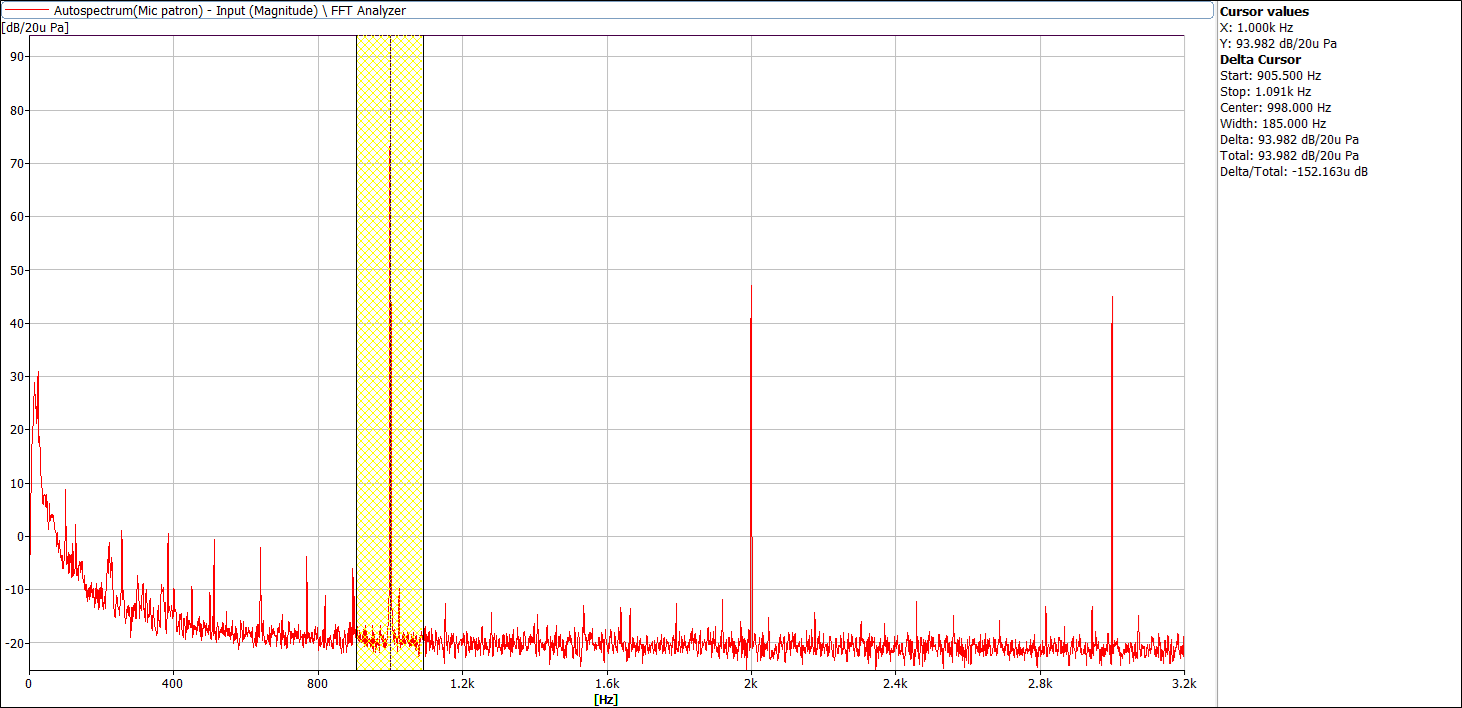
\includegraphics[width=\linewidth]{Imágenes/1. Autoespectro micrófono patrón.png}
  \caption{Autoespectro del micrófono patrón al ser excitado por el calibrador sonoro.}
  \label{fig:Autoespectro_micro_patron}
\end{figure}

El valor medido por el cursor principal es de $L_{\text{main}} = \qty{93.98}{\dB_{\text{SPL}}}$, y resulta que el valor medido por el cursor delta es exactamente el mismo, $L_{\Delta} = \qty{93.98}{\dB_{\text{SPL}}}$. Esto sucede porque prácticamente toda la energía de la señal medida reside en el tono de \qty{1}{\kilo \hertz }. La diferencia entre la energía de ese tono y el resto de frecuencias de la delta es de aproximadamente \qty{110}{\dB}. Al ser tan grande esta diferencia, los valores de la delta apenas aportan energía a la señal, y por tanto el valor de la delta es prácticamente el mismo que el del cursor principal.

\subsection{Proporcionar la sensibilidad del micrófono de prueba medido durante la práctica. Adjuntar las gráficas obtenidas y explicar el procedimiento. Contrastar la sensibilidad con los datos del fabricante (descargar y adjuntar las especificaciones del fabricante).}

El procedimiento seguido para la medida de la sensibilidad del micrófono AKG D230 consiste en excitarlo con un tono puro de \qty{1}{\kilo\hertz} que genere una presión de \qty{1}{\pascal } en su diafragma. Esto es conseguido utilizando un micrófono patrón calibrado con un calibrador sonoro, o bien con un medidor de nivel sonoro de precisión \cite[p.~315]{SSE}. En esta ocasión se ha decidido usar el micrófono patrón. En primer lugar, se emite esta señal con un altavoz y se ajusta su nivel hasta que el micrófono patrón mida \qty{94}{\dB_{\text{SPL}}}. A continuación, se amplifica la señal eléctrica recogida del micrófono de prueba para realizar una medida adecuada. Esta ganancia será tenida en cuenta a la hora de calcular el valor de la sensibilidad. Finalmente, se obtiene la \autoref{fig:Sensibilidad_D230}.

\begin{figure}[hbtp]
  \centering
  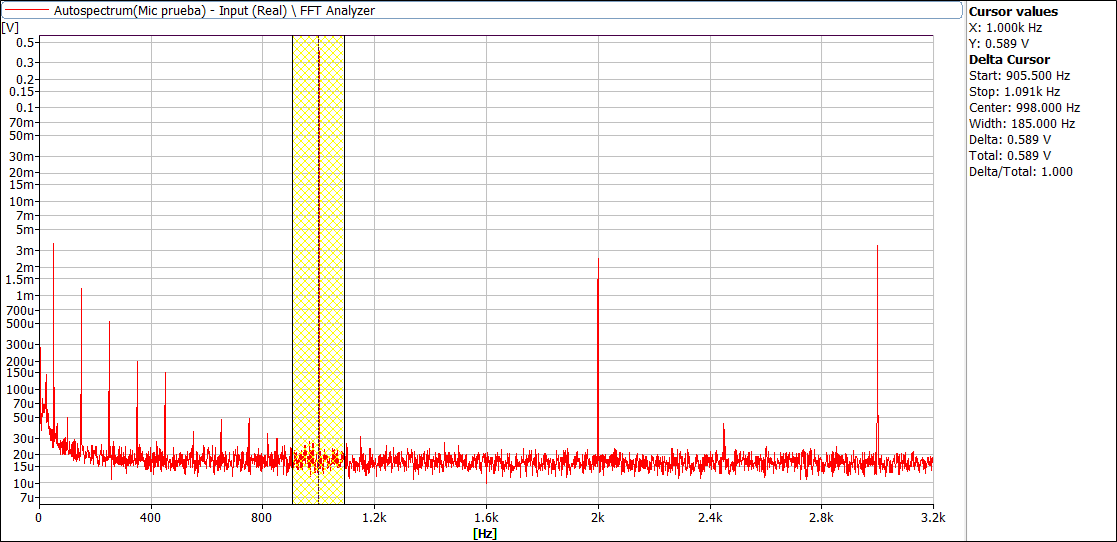
\includegraphics[width=\linewidth]{Imágenes/2. Sensibilidad del micrófono D230.png}
  \caption{Medición de la sensibilidad del micrófono AKG D230.}
  \label{fig:Sensibilidad_D230}
\end{figure}

La medida obtenida es de \qty{0.589}{\volt }. Teniendo en cuenta que la interfaz de audio Motu utilizada aplicó una ganancia de \qty{65}{\dB} a la señal, se puede calcular la sensibilidad del este micrófono como:

\begin{equation} \label{eq:Sensibilidad_D230}
  S = \num{0.589} \cdot 10^{-\frac{65}{20} } = \qty{0.33}{\milli \volt \per \pascal }
\end{equation}

Esta sensibilidad no se corresponde con el valor que proporciona el fabricante, que es de \qty{2.5}{\milli \volt \per \pascal } como se puede ver en la \autoref{fig:datos_fabricante}. La razón de esto es una conexión errónea y/o defectuosa del micrófono al equipo de preamplificación Motu.

\begin{figure}[hbtp]
  \centering
  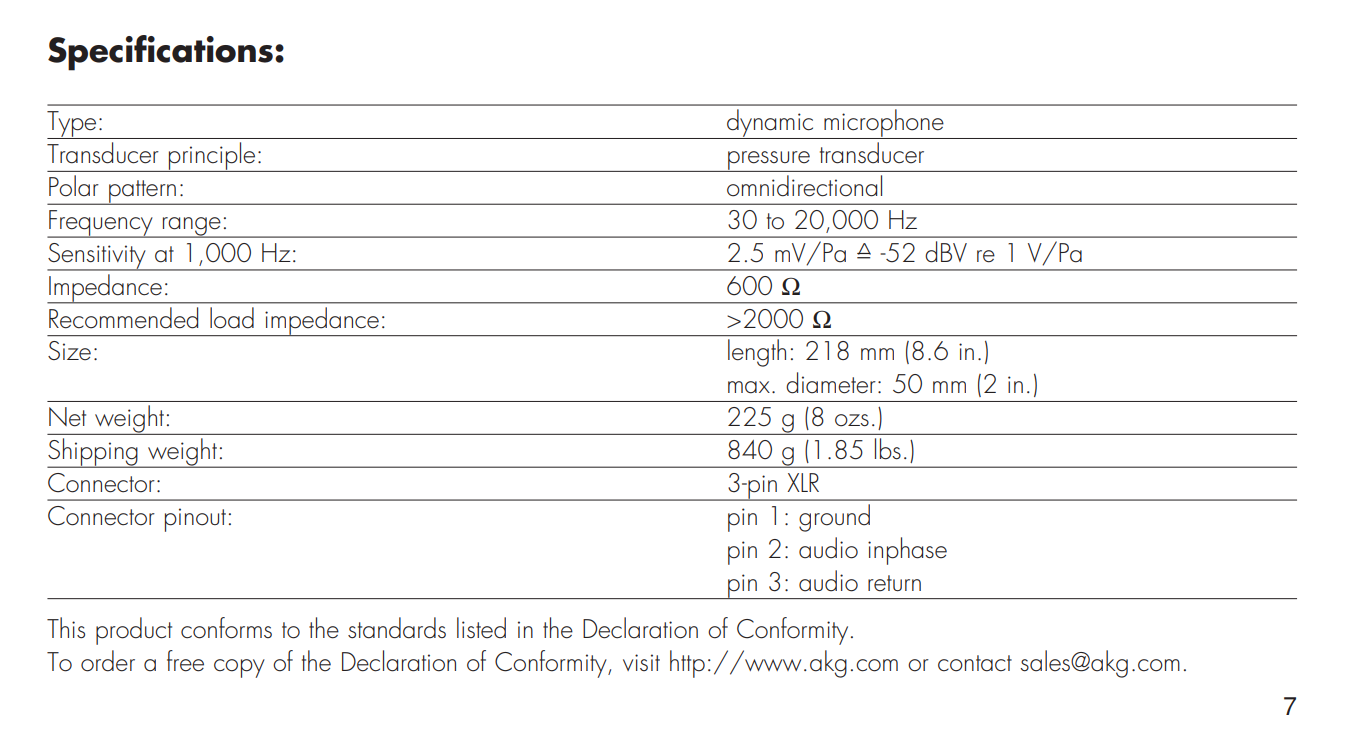
\includegraphics[width=0.8\linewidth]{Imágenes/Datos del fabricante.png}
  \caption{Especificaciones del micrófono AKG D230.}
  \label{fig:datos_fabricante}
\end{figure}


\subsection{Proporcionar la respuesta en frecuencia en campo lejano a 0º y 135º del micrófono de prueba en el intervalo \qty{20}{\hertz } – \qty{20}{\kilo\hertz } (eje $y$ en dB re. \qty{1}{\volt\per\pascal}).}

En la \autoref{fig:grados} se muestra la gráfica requerida. La ganancia del amplificador es de \qty{25}{\dB}.

\begin{figure}[hbtp]
  \centering
  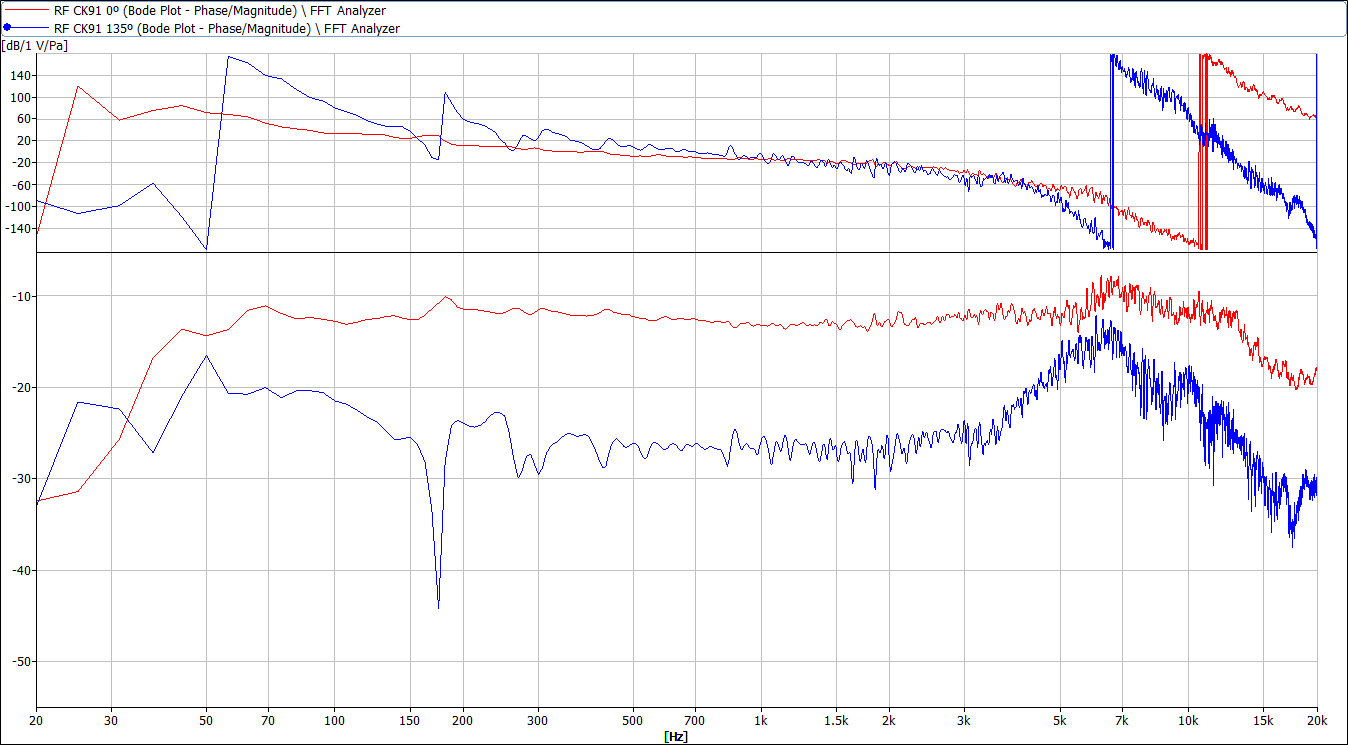
\includegraphics[width=\linewidth]{Imágenes/Micro diferentes angulos.png}
  \caption{Medición de la respuesta en frecuencia del micrófono AKG D230 en campo lejano, a \ang{0} y \ang{135} con respecto a su eje}
  \label{fig:grados}
\end{figure}

\subsubsection{La Sensibilidad en dB re. \qty{1}{\volt\per\pascal}, sólo módulo.}

En la \autoref{tab:sensibilidad} aparecen los datos requeridos, una vez corregido el valor según la ganancia del amplificador.

% Table generated by Excel2LaTeX from sheet 'P2-1 Respuesta en frecuencia'
\begin{table}[htbp]
  \centering
  \caption{Sensibilidad del micrófono AKG D230 en campo lejano}
  \begin{tabular}{|l|r|r|}
    \cline{2-3}    \multicolumn{1}{r}{} & \multicolumn{1}{|l|}{$f = \qty{1}{\kilo \hertz }$} & \multicolumn{1}{l|}{$f = \qty{8}{\kilo \hertz }$} \bigstrut    \\
    \hline
    $S (\ang{0})$                       & \qty{-38.24}{\dB} re. \qty{1}{\volt \per \pascal } & \qty{-36.19}{\dB} re. \qty{1}{\volt \per \pascal }   \bigstrut \\
    \hline
    $S (\ang{135})$                     & \qty{-50.62}{\dB} re. \qty{1}{\volt \per \pascal } & \qty{-45.75}{\dB} re. \qty{1}{\volt \per \pascal }   \bigstrut \\
    \hline
  \end{tabular}%
  \label{tab:sensibilidad}%
\end{table}%



\subsubsection{El módulo de la directividad en dB: $D(\theta = \ang{135}, f) \, [\unit{\dB}]$. Comparar el resultado con la directividad proporcionada por el fabricante (aproximar a las frecuencias disponibles):}

La directividad es fácilmente calculada a partir de la sensibilidad del eje, tomando esta como referencia de \qty{0}{\dB} para cada frecuencia. En la \autoref{tab:Directividad} aparecen los valores requeridos.

% Table generated by Excel2LaTeX from sheet 'P2-1 Respuesta en frecuencia'
\begin{table}[htbp]
  \centering
  \caption{Directividad del micrófono AKG CK 91 en campo lejano}
  \begin{tabular}{|l|r|r|}
    \cline{2-3}    \multicolumn{1}{r}{} & \multicolumn{1}{|l|}{$f = \qty{1}{\kilo \hertz }$} & \multicolumn{1}{l|}{$f = \qty{8}{\kilo \hertz }$} \bigstrut \\
    \hline
    $D (\ang{0})$                       & \qty{0}{\dB}                                       & \qty{0}{\dB}  \bigstrut                                     \\
    \hline
    $D (\ang{135})$                     & \qty{-12.38}{\dB}                                  & \qty{-9.56}{\dB}  \bigstrut                                 \\
    \hline
  \end{tabular}%
  \label{tab:Directividad}%
\end{table}%

En la \autoref{fig:especificaciones_CK91} se muestran las especificaciones que otorga el fabricante sobre la directividad del micrófono AKG CK 91. Se puede comprobar observando las curvas roja y amarilla que los datos de directividad medidos son aproximadamente similares.

\begin{figure}[hbtp]
  \centering
  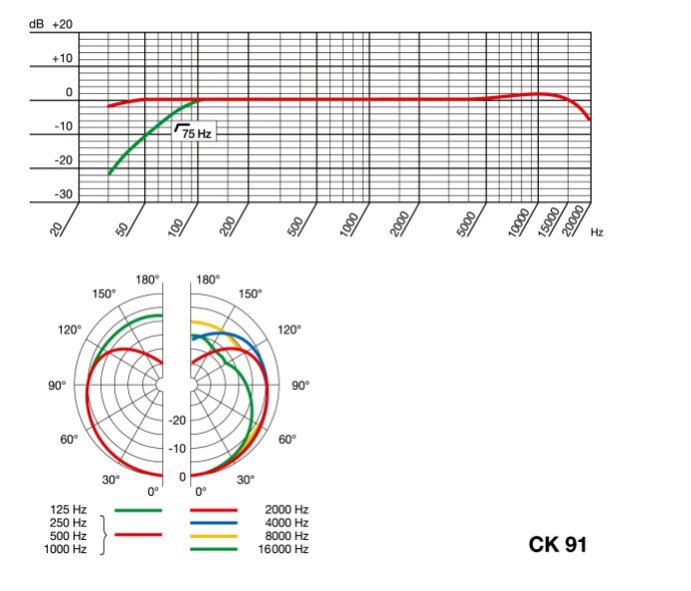
\includegraphics[width=0.6\linewidth]{Imágenes/directividad.png}
  \caption{Especificaciones de directividad del micrófono AKG CK 91}
  \label{fig:especificaciones_CK91}
\end{figure}

\newpage
\bibliography{bibliography}
\bibliographystyle{ieeetran}

\end{document}
